\subsection{符号与组合}

数学理论的符号 \(\mathcal{C}\)\footnote{随着本章的推进，这一表达的含义将变得清晰。} 如下：

\begin{enumerate}
\def\labelenumi{(\arabic{enumi})}
\item
  逻辑符号\footnote{关于这些符号的直观含义，参见第3节，注记。}: \(\square, \tau, \vee, \neg\).
\item
  字母。
\end{enumerate}

所谓字母，我们指的是带或不带重音的大写和小写罗马字母。因此 A、A'、A''、A'''， \ldots{} 都是字母。在文本的任何位置，都可以引入先前论证中未曾出现过的字母。

\begin{enumerate}
\def\labelenumi{(\arabic{enumi})}
\setcounter{enumi}{2}
\tightlist
\item
  特定符号，它们取决于所考虑的理论。
\end{enumerate}

在集合论中，我们将只使用以下三个特定符号： \(=, \in, \supset\) .

\(\mathfrak{C}\) 中的一个组装，是把 \(\mathfrak{C}\) 的若干符号依次并排写成的序列；某些非字母符号可以两两用上方的横线相连，这些横线称为连接线。*例如，在集合论中，\(\in\) 是一个特定符号，

\pandocbounded{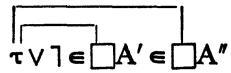
\includegraphics[keepaspectratio]{images/part001_434fa5c1de2e0e5711bd2657d8ea90475ca0e52e33fa2d57a405da317d612ec5.jpg}}

就是一个组装。*

完全使用组装将给印刷者和读者都带来难以克服的困难。因此，现行文本使用不属于形式数学的缩写符号（尤其是日常语言中的词语）。引入此类符号是定义的目的。它们的使用对理论并非必不可少，且常常可能导致混淆，只有读者对主题具备一定熟悉程度才能避免。

\minorheading{示例}

\begin{enumerate}
\def\labelenumi{(\arabic{enumi})}
\item
  组装 \(\vee\neg\) 用 \(\Longrightarrow\) 表示。
\item
  以下符号表示组装（而且是非常长的组装）：
\end{enumerate}

\[
\begin{gathered}
\text{``3 且 4''} \\
\phi \\
\mathbf{N} \\
\mathbf{Z} \\
\text{``实数直线''} \\
\text{``该 }\Gamma\text{ 函数''} \\
f \circ g \\
\pi = \sqrt{2} + \sqrt{3} \\
1 \in 2
\end{gathered}
\]

“每个有限除环都是域”

“\(\zeta(s)\) 的零点，除 \(-2, -4, -6, \ldots\) 之外，位于直线上

\[
\mathcal{R}(s) = 1/2
\]''.

一般来说，用来表示一个组装的符号包含该组装中出现的所有字母。不过，有时也可以违反这一原则而不致混淆。*例如，“X的完备化”表示一个含有字母X的组装，同时还含有另一个字母，用来表示X的一致结构的周围集族。另一方面，

\[
\int_ {0} ^ {1} f (x) d x
\]

表示一个不含字母x（也不含字母d）的组装；N、Z和“Γ函数”所表示的组装也不含任何字母。*

一个数学理论（或简称理论）包含一些规则，这些规则允许我们断言某些符号组合是该理论的项或关系，以及其他规则允许我们断言某些组合是该理论的定理。

本章中对这些规则的描述并不属于形式数学的范畴；这些规则涉及或多或少未确定的组合，例如未确定的字母。为简化表述，我们便于用较不繁琐的符号来指称此类组合。我们将特别使用（数学理论的）符号组合、粗斜体字母（带或不带下标或重音符号）以及特定符号，其中将给出一些示例。由于我们的目的仅在于避免迂回说法（参见§3第1号第28页脚注(*)），我们不会为这些符号的使用制定严格的一般规则；读者在每种具体情况下都能毫无困难地重构所涉及的组合。为用语简便，我们常称这些符号即为组合，而非它们表示组合；因此，在以下规则的陈述中，诸如“组合A”或“字母x”之类的表述，应替换为“由A表示的组合”或“由x表示的字母”。

设 \(A\) 和 \(B\) 为组装。用 \(AB\) 表示把组装 \(B\) 写在组装 \(A\) 右边所得的组装。用 \(\vee A \neg B\) 表示从左到右依次写下符号 \(\vee\) 、组装 \(A\) 、符号 \(\neg\) 和组装 \(B\) 所得的组装。其余类推。

设 \(A\) 为一个组装，\(x\) 为一个字母。用 \(\tau_{x}(A)\) 表示按如下方式构造的组装：先形成组装 \(\tau A\) ，把 \(x\) 在 \(A\) 中的每一处出现与 \(\tau\) 相连，后者写在 \(A\) 左侧；再把每一处 \(x\) 都换成符号 \(\square\) 。因此，\(\tau_{x}(A)\) 所表示的组装不含 \(x\) 。

例。符号 \(\tau_{x}(\in xy)\) 表示组装

\[
\tau \in \square y.
\]

设A和B为组装，x为一个字母。将A中所有出现的x替换为组装B所得的组装记为 \((B|x)A\) （读作：B 在 A 中替换 x）。如果 x 不出现在 A 中，则 \((B|x)A\) 与 A 相同；特别地，

\[
(B | \boldsymbol {x}) \tau_ {\boldsymbol {x}} (A)
\]

与 \(\tau_{\mathbf{x}}(A)\) 相同。

例。若将 \(x\) 替换为 \(\square\) ，每逢 \(x\) 在组装 \(\vee \in xy = xx\) 中出现便作此替换，就得到组装 \(\vee \in \square y = \square \square\) 。

若 \(A\) 是一个组装，而我们特别关注一个字母 \(x\) ，或两个不同的字母 \(x\) 和 \(y\) （它们可以出现或不出现在 \(A\) 中），则常写作 \(A \{x\}\) 或 \(A \{x, y\}\) 。在这种情况下，用 \(A \{B\}\) 代替 \((B|x)A\) 。用 \(A \{B, C\}\) 表示同时把 \(x\) 换成 \(B\) 、把 \(y\) 换成 \(C\) （每逢它们在 \(A\) 中出现便作替换；注意，\(x\) 和 \(y\) 可以出现在 \(B\) 及 \(C\) 中）；若 \(x'\) 和 \(y'\) 是不同于 \(x\) 和 \(y\) 的两个不同字母，并且均不出现在 \(A, B\) 或 \(C\) 中，则 \(A \{B, C\}\) 与 \((B|x') (C|y') (x'|x) (y'|y)A\) 相同。

备注。当引入一个缩写符号 \(\Sigma\) （借助定义）用以表示某个组装时，通常（隐含地）约定：将原组装中的字母x替换为组装B所得到的组装，用将 \(\Sigma\) 中的字母x替换为组装B（或更常见地，替换为表示组装B的缩写符号）后所得的符号来表示。

¶ *例如，一旦定义了由符号E⊗F所表示的组装——其中E和F是字母，这个组装此外还包含除E和F之外的其他字母——符号Z⊗F就可以无需进一步解释地使用。*

¶ 这条规则可能会导致混淆，而通过使用各种排版手段可以避免这些混淆；最常见的方法是用 (B) 替换 x 来代替 B。

¶ *例如，M∩N 表示一个包含字母 N 的组装。如果我们用 P∪Q 所表示的组装替换 N，则得到由 M∩(P∪Q) 表示的组装。*

